\chapter{Some useful formulas of atomic physics}

\section{Relationship between measurement strength and scattering rates}
To avoid using reduced dipole moment elements and other quantities in a wrong unit, we can normalize some quantities in terms of characteristic scattering rates and field intensities.
Here are some basic relationships.

Starting from the saturation parameter,
\begin{align}
S(\Delta ) &\equiv \frac{\Omega^2/2}{\Delta^2+\frac{\Gamma^2}{4}} = \frac{S(0)}{4\Omega^2/\Gamma^2+1} \approx \frac{\Omega^2}{2\Delta^2} \quad (\text{for $\Delta^2\gg \Gamma^2$})\\
S(0) &= \frac{I}{I_{\rm sat}}= \frac{2\Omega^2}{\Gamma^2}\\
I_{\rm sat} &= \frac{\hbar \omega}{\sigma_0} \frac{\Gamma}{2}.\label{eq:Isatsigma0}
\end{align}
Therefore, 
\begin{align}\label{eq:OmegaGamma}
\Omega^2 &= \frac{I}{I_{\rm sat}}\frac{\Gamma^2}{2}.
\end{align}


If we define a characteristic scattering rate as
\begin{align}
\gamma_s &\equiv \frac{\Gamma \Omega^2}{4\Delta_{\rm eff}^2},
\end{align}
then the relationships we have derived above (Eqs.~\ref{eq:OmegaGamma} and~\ref{eq:Isatsigma0}) will lead to
\begin{align}
\gamma_s &= \frac{\Gamma^3}{8\Delta_{\rm eff}^2} \frac{I}{I_{\rm sat}}\\
&= \sigma_0 \frac{\Gamma^2}{4\Delta_{\rm eff}^2}\frac{I}{\hbar \omega}.
\end{align}
This final step matches with the physical definition of $ \gamma_s $ that 
\begin{align}
\gamma_s &\equiv N_e \Gamma =\frac{S(\Delta_{\rm eff})}{2} \Gamma\\
&\equiv \sigma(\Delta_{\rm eff}) \frac{I}{\hbar \omega},
\end{align}
where $ \sigma(\Delta)=\frac{\sigma_0}{1+\frac{4\Delta^2}{\Gamma^2}}\approx \sigma_0 \frac{\Gamma^2}{4\Delta^2} $.

We define $ I=\frac{P}{A_{\rm in}}= \frac{\hbar \omega }{A_{\rm in}} \dot{N}_L $, and then
\begin{align}
\gamma_s &= \frac{\sigma_0 }{A_{\rm in}} \frac{\Gamma^2}{4\Delta_{\rm eff}^2}\dot{N}_L.
\end{align}

In a typical spin-squeezing case, the measurement strength may be given by
\begin{align}
\kappa &= \chi_{\rm eff}^2 \dot{N}_L,
\end{align} 
where $ \chi_{\rm eff}= \frac{\sigma_0}{A_{\rm eff}} \frac{\Gamma}{4\Delta_{\rm eff}} $.
Therefore,
\begin{align}
\kappa &= \frac{\sigma_0^2}{A_{\rm eff}^2} \frac{\Gamma^2}{16 \Delta_{\rm eff}^2} \dot{N}_L 
= \frac{A_{\rm in}\sigma_0}{4 A_{\rm eff}^2}\gamma_s.
\end{align}


As an example of spin-squeezing parameter calculation using the formulas above, we plot in Fig.~\ref{fig:QNDproperty_magic44} the optimal peak spin squeezing parameter (with various atom numbers) and OD-related parameters.

\begin{figure}
\begin{minipage}{.49\linewidth}
\centering
\subfloat[]{\label{fig:xi_optimal_NA1000to5000_omega44}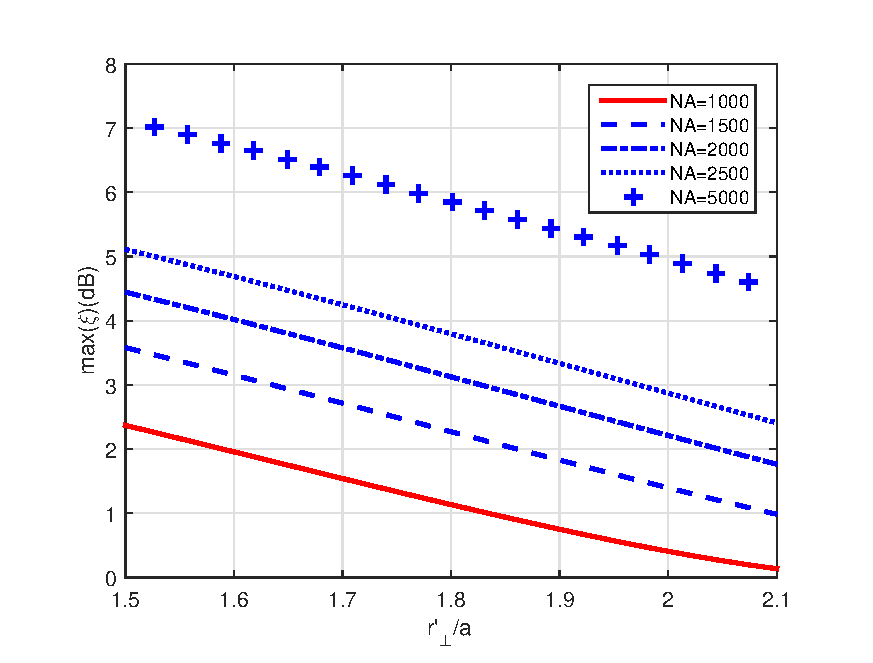
\includegraphics[scale=0.45]{./Figs/xi_optimal_NA1000to5000_omega44}}
\end{minipage}
\begin{minipage}{.49\linewidth}
\centering
\subfloat[]{\label{fig:OD_optimal_rp}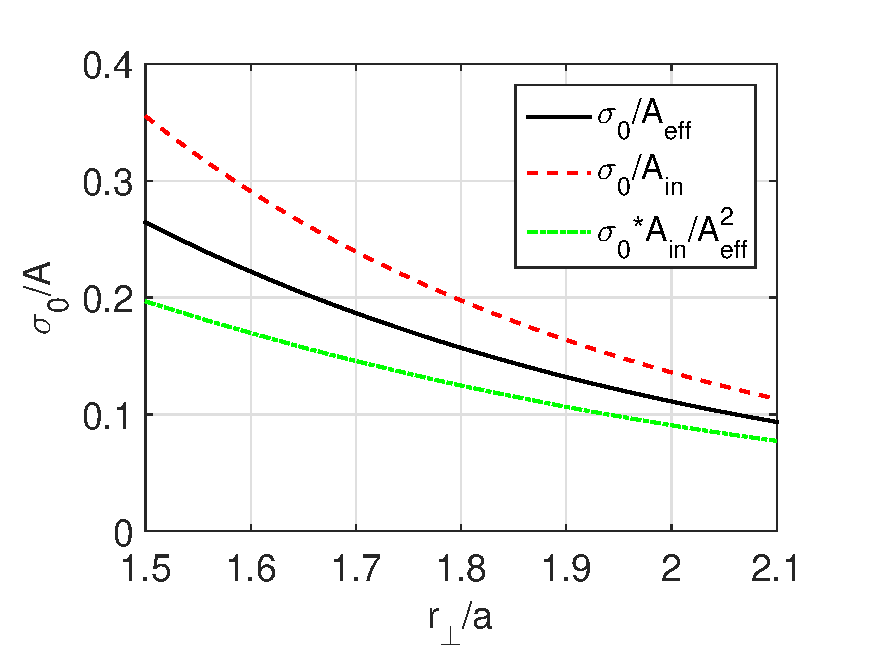
\includegraphics[scale=0.45]{./Figs/OD_optimal_rp}}
\end{minipage}
\caption{QND measurement properties using the magic frequency $ \omega_{44} $. Subfigure~\protect\subref{fig:xi_optimal_NA1000to5000_omega44} shows the optimal peak spin squeezing parameter as a function of the radial position of the atom. Different atom numbers have been indicated in different types of lines. Subfigure~\ref{fig:OD_optimal_rp} shows the OD per atom parameters and the ratio of $ 4\kappa/\gamma_s $ as a function of atoms' radial position when the optimal quantization axis is chosen to plot Subfig.~\protect\subref{fig:xi_optimal_NA1000to5000_omega44}.}\label{fig:QNDproperty_magic44}
\end{figure}
